% AgentScript: IEEE conference-format technical report.
% Compile with pdfLaTeX (for example on Overleaf). Generated from the same content as
% AgentScript-IEEE.docx; every listing is pasted from a real run of the compiler.
\documentclass[conference]{IEEEtran}
\IEEEoverridecommandlockouts
\usepackage[T1]{fontenc}
\usepackage[utf8]{inputenc}
\usepackage{textcomp}
\usepackage{cite}
\usepackage{amsmath,amssymb}
\usepackage{array}
\usepackage{xcolor}
\usepackage{listings}
\usepackage{tikz}
\usetikzlibrary{arrows.meta,positioning,fit,backgrounds}
\usepackage[hyphens]{url}
\lstset{basicstyle=\ttfamily\footnotesize, columns=fixed, basewidth=0.5em, keepspaces=true,
  breaklines=true, breakatwhitespace=false, showstringspaces=false, upquote=true,
  postbreak=\mbox{\textcolor{gray}{$\hookrightarrow$}\space}, aboveskip=2pt, belowskip=2pt,
  xleftmargin=0pt, frame=none}
\newcolumntype{P}[1]{>{\raggedright\arraybackslash}p{#1}}
\begin{document}
\title{AgentScript: Compile-Time Taint and Approval Checking for Safe AI-Agent Programs}
\author{\IEEEauthorblockN{Ashvik Mishra}
\IEEEauthorblockA{\textit{Compiler Design Laboratory Project}\\
ashvikmishra.mit@gmail.com}}
\maketitle

\begin{abstract}
Agents built on large language models (LLMs) call tools such as web search, e-mail and the file system, and agent frameworks typically check safety at run time, if at all, so a mistake surfaces only after a tool has already fired. This paper presents AgentScript, a deliberately tiny agent language and a ten-stage compiler written in Python that rejects unsafe agent programs before they run. Trust decisions live in a fixed, built-in tool annotation table rather than in program syntax. A forward data-flow taint analysis over the control-flow graph (CFG) of the unoptimized intermediate representation proves that untrusted data never reaches a privileged tool without passing through a sanitizer, and an approval analysis based on dominators proves that every irreversible call is dominated by the ``yes'' branch of a human confirmation. Permission lists and a worst-path call budget are checked during semantic analysis and enforced again by a stack virtual machine. Optimization (constant folding, dead-code elimination and a restricted duplicate tool-call elimination) runs only after every safety check has passed; on the demonstration program it reduces tool calls from 4 to 2, and an optional scheduler groups independent calls into parallel rounds (4 rounds to 2). The implementation passes 941 tests, and each of its 14 demonstrable error codes has its own failing example program.
\end{abstract}

\begin{IEEEkeywords}
compilers, static analysis, taint analysis, information-flow control, dominators, domain-specific languages, LLM agents, prompt injection
\end{IEEEkeywords}

\section{Introduction}
An LLM agent is a program that calls tools: a web search, a language model, e-mail, the file system. Agent frameworks typically check safety at run time, if at all, so a mistake is noticed only after a tool has fired. Three failure modes matter most. \emph{Prompt injection}: text fetched from the web or a file contains instructions, and the agent passes it into a powerful tool such as \texttt{send\_email}~\cite{greshake}, \cite{owasp}. \emph{Irreversible actions}: the agent deletes a file with no human confirmation. \emph{Unbounded tool use}: the agent loops or repeats identical calls, wasting money and hitting rate limits.

The first two are questions about data flow (where can a value travel?) and control flow (which paths reach this call?), which compilers have answered with static analysis for decades~\cite{aho}. AgentScript therefore moves the checks from run time to compile time: a program that could leak web content into \texttt{send\_email}, or delete a file on a path where nobody said yes, does not compile, and the programmer receives an error with a line, a column and the offending path. The third failure mode is reduced rather than proved away, by a \texttt{permit} list, a call \texttt{budget} and duplicate-call elimination.

The language is deliberately tiny so that these properties stay simple and exact: a fixed set of seven built-in tools, immutable variables, no functions, no task-to-task calls and one bounded loop form. The contributions are:

\begin{enumerate}
\item a small agent language whose trust policy is a fixed tool-annotation table, plus \texttt{permit} and \texttt{budget} declarations checked statically and again at run time;
\item a compile-time taint analysis over the CFG that reports untrusted-to-privileged flows (E401) with the full source-to-sink path;
\item an approval analysis that uses dominators and \emph{guard blocks} to prove that every irreversible call follows a ``yes'' from \texttt{confirm}, distinguishing a missing confirmation (E501) from one that does not guard every path (E502);
\item a complete classic pipeline (lexer to stack VM) with an ordering rule that runs every safety analysis on the unoptimized program, an effect-aware optimizer and an optional parallel scheduler that never reorders barrier tools;
\item a web editor that shows every stage's output, and an evaluation with 941 passing tests and a failing demo program for each of 14 error codes.
\end{enumerate}

Section II reviews related work, Section III presents the language, Section IV the compiler architecture, Section V the two safety analyses and Section VI optimization, code generation and scheduling. Sections VII to X cover the implementation, evaluation, limitations and conclusions.

\section{Related Work}
\emph{LLM programming tools.} DSPy~\cite{dspy} builds LLM pipelines from declarative modules and optimizes their prompts automatically. LMQL~\cite{lmql} is a query language that constrains what a model generates. Guidance~\cite{guidance} offers templating and constrained generation, and BAML~\cite{baml} is a domain-specific language for typed LLM functions with structured outputs. These tools are about prompting and output structure; none of them checks, before execution, where data flows between tools or which paths reach a side effect.

\emph{Prompt injection.} Greshake \emph{et al.}~\cite{greshake} showed that instructions planted in retrieved content can take over LLM-integrated applications (indirect prompt injection), and prompt injection heads the OWASP list of risks for LLM applications~\cite{owasp}. CaMeL~\cite{camel} defends agents by design, separating trusted control flow from untrusted data and enforcing policies when tools are called. AgentScript makes a similar separation but checks it statically: an unsafe program is rejected before any tool runs.

\emph{Taint analysis and information-flow control.} Denning's lattice model~\cite{denning} is the basis of information-flow control; Sabelfeld and Myers~\cite{sabelfeld} survey language-based enforcement, including implicit flows through branches, and JFlow~\cite{jflow} brought static checking to a mainstream language. Static taint analysis finds injection vulnerabilities in web applications~\cite{livshits}. AgentScript uses the simplest instance: a two-point lattice, explicit flows only, with agent tools as sources, sanitizers and sinks.

\emph{Control-flow analysis and dominators.} Allen~\cite{allen} formalized control-flow analysis and Kildall~\cite{kildall} the iterative data-flow framework used here for taint. Dominators can be computed in near-linear time by Lengauer and Tarjan~\cite{lt}; Cooper, Harvey and Kennedy~\cite{cooper} showed that a carefully engineered iterative algorithm is competitive in practice. AgentScript's CFGs have a handful of blocks, so it uses the simple set-based iterative algorithm of the Dragon Book~\cite{aho}.

\emph{Capabilities and effects.} The \texttt{permit} list is a capability list in the sense of Dennis and Van Horn~\cite{dennis} and of object-capability systems~\cite{miller}; the \texttt{privileged} and \texttt{irreversible} flags are effect annotations on tools, related to effect systems~\cite{lucassen}. The novelty of AgentScript is not any one technique but their combination in a small, working compiler for agent programs.

\section{Language Design}
A program is one agent with zero or more \texttt{permit} lines, exactly one \texttt{budget}, and one or more tasks. A task has typed parameters, a return type and a block of statements: \texttt{let}, \texttt{if}/\texttt{else}, \texttt{repeat}, \texttt{return} and expression statements. Fig.~\ref{fig:source} shows the running example, which searches the web, sanitizes the first result, summarizes it with the LLM and e-mails the summary only after a confirmation.

\begin{figure}[!htb]
\begin{lstlisting}
agent Assistant {
  permit web_search, llm, sanitize, send_email, confirm;
  budget calls = 5;

  task report(topic: string) -> bool {
    let raw = web_search(topic);
    let clean = sanitize(raw[0]);
    let summary = llm("Summarize: " + clean);
    if (confirm("Send report?")) {
      return send_email("me@example.com", summary);
    }
    return false;
  }
}
\end{lstlisting}
\caption{The running example, examples/valid\_report.as.}
\label{fig:source}
\end{figure}

\subsection{Syntax}
The parser implements exactly the EBNF of the specification and nothing more; Fig.~\ref{fig:grammar} shows an excerpt (expression levels for equality, relational, additive and multiplicative operators are omitted). All binary operators are left-associative. Deliberately absent are assignment, \texttt{else if}, \texttt{!}, \texttt{\&\&}, \texttt{||}, \texttt{/\allowbreak{}}, unary minus, list literals, user functions and task-to-task calls. Without \texttt{\&\&} and \texttt{||} there is no short-circuit control flow hidden inside expressions, so the CFG comes only from \texttt{if} and \texttt{repeat}; immutable variables give each IR variable one static definition. The lexer lexes \texttt{\textgreater{}\textgreater{}} as two \texttt{\textgreater{}} tokens so that \texttt{list\textless{}list\textless{}string\textgreater{}\textgreater{}} works, and the parser reports only the first syntax error (E201), with no recovery. Nesting is bounded at 1000 levels.

\begin{figure}[!htb]
\begin{lstlisting}
program     = "agent" IDENT "{" { permit_decl }
              budget_decl task { task } "}" EOF ;
permit_decl = "permit" IDENT { "," IDENT } ";" ;
budget_decl = "budget" "calls" "=" INT ";" ;
task        = "task" IDENT "(" [ param { "," param } ]
              ")" "->" type block ;
type        = "string" | "int" | "bool"
            | "list" "<" type ">" ;
statement   = let_stmt | if_stmt | repeat_stmt
            | return_stmt | expr_stmt ;
let_stmt    = "let" IDENT "=" expr ";" ;
if_stmt     = "if" "(" expr ")" block [ "else" block ] ;
repeat_stmt = "repeat" ( INT | IDENT ) block ;
postfix     = primary { "[" expr "]" } ;
primary     = INT | STRING | "true" | "false"
            | IDENT [ "(" [ expr { "," expr } ] ")" ]
            | "(" expr ")" ;
\end{lstlisting}
\caption{Grammar excerpt (EBNF, from the specification).}
\label{fig:grammar}
\end{figure}

\subsection{Types and Scopes}
The types are \texttt{string}, \texttt{int}, \texttt{bool} and \texttt{list\textless{}T\textgreater{}}; \texttt{let} infers its type from the initializer. Every value also carries a hidden taint label, \texttt{trusted} or \texttt{untrusted}, and a list carries one label for all its elements. Scopes nest builtins $\rightarrow$ agent $\rightarrow$ task $\rightarrow$ block. There is no shadowing: declaring a name already visible in this or any enclosing scope is E302, so a name means one thing throughout a task. Every task must return on every path (E304); \texttt{repeat} never counts as returning because it may run zero times.

\subsection{Built-in Tools}
Table~\ref{tab:tools} lists the seven tools and their flags. Annotations are not syntax: a program cannot declare a tool or change a flag. The guarantees are only as good as the annotations, and if programs could write their own, a program could simply mark \texttt{web\_search} as trusted. A fixed table keeps every trust decision in one reviewed file.

\begin{table}[!htb]
\caption{Built-in Tool Table (Fixed in agentscript/tools.py)}
\label{tab:tools}
\centering
\footnotesize
\setlength{\tabcolsep}{3pt}
\renewcommand{\arraystretch}{1.1}
\begin{tabular}{P{0.765in}P{1.165in}P{1.315in}}
\hline
\textbf{Tool} & \textbf{Signature} & \textbf{Flags} \\
\hline
\texttt{web\_search} & (string) $\rightarrow$ list\textless{}string\textgreater{} & untrusted\_result, mergeable \\
\texttt{read\_file} & (string) $\rightarrow$ string & untrusted\_result, mergeable \\
\texttt{llm} & (string) $\rightarrow$ string & propagates\_taint, mergeable \\
\texttt{sanitize} & (string) $\rightarrow$ string & sanitizer, mergeable \\
\texttt{send\_email} & (string, string) $\rightarrow$ bool & privileged \\
\texttt{delete\_file} & (string) $\rightarrow$ bool & privileged, irreversible \\
\texttt{confirm} & (string) $\rightarrow$ bool & approval \\
\hline
\end{tabular}
\end{table}
\subsection{Permissions and Budget}
Calling a tool that no \texttt{permit} line lists is E305. The declaration \texttt{budget calls = N} applies to each task run, and every call counts as one, including \texttt{sanitize} and \texttt{confirm}. The static count is the worst path over the AST: a sequence sums its statements, an \texttt{if} counts its condition plus the larger branch, and \texttt{repeat n} with a literal \texttt{n} multiplies its body by \texttt{n}. If the count exceeds the budget, E306 is reported at the (budget+1)-th call on the worst path (Fig.~\ref{fig:e306}). A \texttt{repeat x} with a variable count is counted once with warning W306, and the VM enforces the budget on every call (E601).

\begin{figure}[!htb]
\begin{lstlisting}
E306 [semantic] 9:12: task 'dig' may make 4 tool calls on its worst path, but the budget is 3
    6:13  call 1: web_search
    7:13  call 2: web_search
    8:13  call 3: web_search
    9:12  call 4: llm (over budget)
\end{lstlisting}
\caption{E306 for sem\_budget.as (diagnostics section of the compile output).}
\label{fig:e306}
\end{figure}

\section{Compiler Architecture}
Fig.~\ref{fig:pipeline} shows the ten stages: a front end (lexer, parser, semantic analysis), a middle end (IR and CFG, taint, approval, optimizer, scheduler) and a back end (code generation and VM). The six classic phases are stages 1, 2, 3, 4, 7 and 9; stage 8 is the optional M7 milestone, and without it the optimized IR goes straight to code generation.

\begin{figure}[!t]
\centering
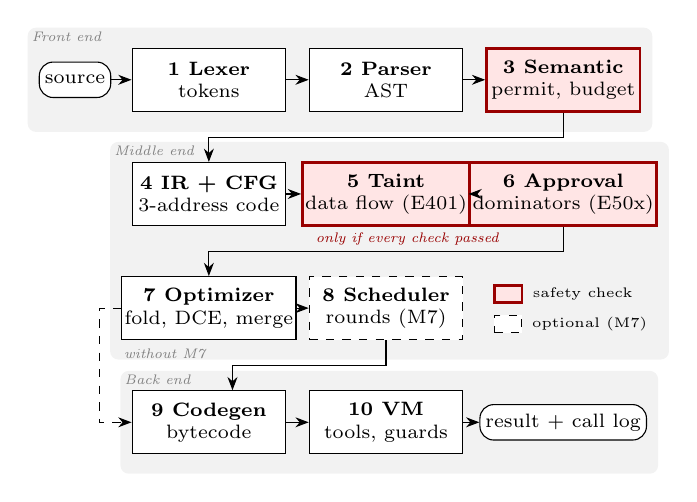
\begin{tikzpicture}[font=\scriptsize, >=Stealth,
  stage/.style={draw, minimum width=1.95cm, minimum height=0.8cm, align=center, fill=white, inner sep=1pt},
  safe/.style={stage, draw=red!60!black, fill=red!10, line width=0.9pt},
  opt/.style={stage, dashed},
  term/.style={draw, rounded corners=5pt, minimum height=0.45cm, align=center, fill=white, inner sep=2pt},
  band/.style={fill=gray!10, rounded corners=3pt, inner xsep=4pt, inner ysep=7pt},
  bandlabel/.style={anchor=north west, font=\tiny\itshape, text=gray, inner sep=1.5pt}]
\node[term] (src) at (0.05,0) {source};
\node[stage] (s1) at (1.75,0) {\textbf{1 Lexer}\\tokens};
\node[stage] (s2) at (4.0,0) {\textbf{2 Parser}\\AST};
\node[safe] (s3) at (6.25,0) {\textbf{3 Semantic}\\permit, budget};
\node[stage] (s4) at (1.75,-1.45) {\textbf{4 IR + CFG}\\3-address code};
\node[safe] (s5) at (4.0,-1.45) {\textbf{5 Taint}\\data flow (E401)};
\node[safe] (s6) at (6.25,-1.45) {\textbf{6 Approval}\\dominators (E50x)};
\node[stage] (s7) at (1.75,-2.9) {\textbf{7 Optimizer}\\fold, DCE, merge};
\node[opt] (s8) at (4.0,-2.9) {\textbf{8 Scheduler}\\rounds (M7)};
\node[stage] (s9) at (1.75,-4.35) {\textbf{9 Codegen}\\bytecode};
\node[stage] (s10) at (4.0,-4.35) {\textbf{10 VM}\\tools, guards};
\node[term] (res) at (6.25,-4.35) {result + call log};
\draw[->] (src) -- (s1);
\draw[->] (s1) -- (s2);
\draw[->] (s2) -- (s3);
\draw[->] (s3.south) -- ++(0,-0.32) -| (s4.north);
\draw[->] (s4) -- (s5);
\draw[->] (s5) -- (s6);
\draw[->] (s6.south) -- ++(0,-0.32) -| node[pos=0.22, above=-1pt, font=\tiny\itshape, text=red!60!black] {only if every check passed} (s7.north);
\draw[->] (s7) -- (s8);
\draw[->] (s8.south) -- ++(0,-0.32) -| ([xshift=3mm]s9.north);
\draw[->, dashed] (s7.west) -- ++(-0.28,0) |- (s9.west);
\node[font=\tiny\itshape, text=gray, anchor=west] at (0.55,-3.5) {without M7};
\draw[->] (s9) -- (s10);
\draw[->] (s10) -- (res);
\node[safe, minimum width=0.35cm, minimum height=0.22cm] (lg1) at (5.55,-2.72) {};
\node[anchor=west, font=\tiny] at (lg1.east) {safety check};
\node[opt, minimum width=0.35cm, minimum height=0.22cm] (lg2) at (5.55,-3.1) {};
\node[anchor=west, font=\tiny] at (lg2.east) {optional (M7)};
\begin{scope}[on background layer]
\node[band, fit=(src)(s1)(s3)] (fe) {};
\node[bandlabel] at (fe.north west) {Front end};
\node[band, fit=(s4)(s6)(s7)(s8)(lg2)] (me) {};
\node[bandlabel] at (me.north west) {Middle end};
\node[band, fit=(s9)(s10)(res)] (be) {};
\node[bandlabel] at (be.north west) {Back end};
\end{scope}
\end{tikzpicture}
\caption{The ten-stage pipeline. Shaded stages run safety checks; all of them precede the optimizer. The dashed stage is the optional scheduler.}
\label{fig:pipeline}
\end{figure}

\emph{Artifacts.} Every compile-time stage produces an artifact of the same shape, \texttt{\{\textquotedbl{}text\textquotedbl{}: ...,\allowbreak{} \textquotedbl{}data\textquotedbl{}: ...\}}: the CLI prints \texttt{text}, the editor renders \texttt{data} (for example the CFG as a Mermaid graph) and golden tests compare \texttt{text}. The compile result holds one artifact per key, \texttt{tokens}, \texttt{ast}, \texttt{symbols}, \texttt{ir}, \texttt{cfg}, \texttt{taint}, \texttt{approval}, \texttt{optimized\_ir}, \texttt{schedule} and \texttt{bytecode}, with \texttt{null} for stages that did not run. The compiler stops at the first error, so every phase reports at most one; warnings never stop it. Every diagnostic has a phase, code, severity, message, line, column and optional path, printed as \texttt{E401 [taint] 9:14: ...} followed by one line per path step.

\emph{Ordering rule.} Every safety analysis (permission, budget, taint, approval) runs on the unoptimized program, and the optimizer runs only after all of them pass, so a guarantee never depends on what the optimizer removes. In \texttt{if (debug) \{ delete\_file(p); \}} with \texttt{debug = false} the optimizer deletes the branch; checking afterwards would accept an unconfirmed \texttt{delete\_file} that is one edit away from running.

\emph{IR and CFG.} Stage 4 lowers the AST to three-address code (Fig.~\ref{fig:ir}). The instructions are \texttt{Assign}, \texttt{BinOp}, \texttt{Index}, \texttt{Call}, \texttt{Jump}, \texttt{Branch}, \texttt{Return}, \texttt{Label} and, with M7, \texttt{ParallelCalls}; every operand is a constant or a variable, and every instruction keeps the line and column of its source construct so that later phases can report errors in source terms. The code is split into basic blocks; for a \texttt{Branch}, the successors are ordered [true, false], which the approval analysis relies on.

\begin{figure}[!htb]
\begin{lstlisting}
task report(topic: string) -> bool
      raw = call web_search(topic)             ; line 6
      t1 = raw[0]                              ; line 7
      clean = call sanitize(t1)                ; line 7
      t2 = "Summarize: " + clean               ; line 8
      summary = call llm(t2)                   ; line 8
      t3 = call confirm("Send report?")        ; line 9
      if t3 goto L1 else L2                    ; line 9
  L1:
      t4 = call send_email("me@example.com", summary) ; line 10
      return t4                                ; line 10
  L2:
      return false                             ; line 12
\end{lstlisting}
\caption{Unoptimized IR of valid\_report.as (compile -{}-phase ir).}
\label{fig:ir}
\end{figure}

\section{Safety Analyses}
\subsection{Taint Analysis}
Labels form a two-point lattice in which \texttt{trusted} lies below \texttt{untrusted}; the join is \texttt{untrusted} if either side is. The analysis is a forward \emph{may} analysis over each task's CFG~\cite{kildall}: the state at a program point is the set of untrusted variables, each with its provenance (the source call and every step since). Table~\ref{tab:transfer} gives the transfer function. At a join a variable is untrusted if it is untrusted on any incoming path:

\begin{equation}
\mathit{IN}[b] = \bigcup_{p \in \mathit{pred}(b)} \mathit{OUT}[p], \qquad \mathit{OUT}[b] = f_b(\mathit{IN}[b])
\end{equation}
\noindent with \texttt{IN[entry]} empty, because task parameters are trusted. Because \texttt{repeat} creates back edges, the blocks are visited round-robin until the set of untrusted variables at every block entry stops changing. The transfer function is monotone and the sets only grow, so the loop stops after at most |vars| $\times$ |blocks| changes. Provenance is taken from the first predecessor that supplies it, which makes the reported path deterministic.

\begin{table}[!htb]
\caption{Taint Transfer Function (Const Operands Are Trusted)}
\label{tab:transfer}
\centering
\footnotesize
\setlength{\tabcolsep}{3pt}
\renewcommand{\arraystretch}{1.1}
\begin{tabular}{P{1.615in}P{1.715in}}
\hline
\textbf{IR instruction} & \textbf{Label of the destination} \\
\hline
\texttt{x = y} (copy) & label of \texttt{y} \\
\texttt{x = a op b} (any operator) & join of \texttt{a} and \texttt{b} \\
\texttt{x = a[i]} & join of \texttt{a} and \texttt{i} \\
call to \texttt{web\_search}, \texttt{read\_file} & untrusted (a new source) \\
call to \texttt{llm} & join of its arguments \\
call to \texttt{sanitize} & trusted \\
any other call & trusted (bool results) \\
\texttt{goto}, branch, \texttt{return} & no change (no implicit flows) \\
\hline
\end{tabular}
\end{table}
\emph{Sink rule.} An untrusted argument to a \texttt{privileged} tool is E401, reported at the sink. For \texttt{valid\_report.as} the analysis reaches its fixed point after two iterations: \texttt{raw} and \texttt{t1} are untrusted, \texttt{clean} is the result of \texttt{sanitize} and therefore trusted, and the \texttt{send\_email} sink is \texttt{OK}. In \texttt{taint\_injection.as}, line 7 passes \texttt{raw[0]} straight to \texttt{llm}. Fig.~\ref{fig:taint} shows the real report: the path reads from source to sink, through the index at 7:42, the concatenation at 7:37 and \texttt{llm} at 7:19, into argument 2 of \texttt{send\_email} at 9:14.

\begin{figure}[!htb]
\begin{lstlisting}
task report  (fixed point after 2 iteration(s))
  untrusted variables:
    raw          line 6    from web_search (line 6)
    t1           line 7    from web_search (line 6)
    t2           line 7    from web_search (line 6)
    summary      line 7    from web_search (line 6)
  sanitized (trusted) results:
    (none)
  privileged sinks:
    send_email line 9  ["me@example.com": trusted, summary: untrusted from web_search]  VIOLATION

E401 [taint] 9:14: untrusted data from web_search (line 6) reaches privileged tool 'send_email' (line 9), argument 2; pass it through sanitize first
    6:15  raw = call web_search(topic)  <- web_search returns untrusted data
    7:42  t1 = raw[0]
    7:37  t2 = "Summarize: " + t1
    7:19  summary = call llm(t2)
    9:14  t4 = call send_email("me@example.com", summary)  <- privileged sink
\end{lstlisting}
\caption{Taint report and E401 for taint\_injection.as (taint section of the compile output).}
\label{fig:taint}
\end{figure}

\subsection{Approval Analysis}
Being dominated by the \texttt{confirm} call is not enough, because \texttt{confirm} can return false: in \texttt{let ok = confirm(..); delete\_file(p);} the confirm dominates the deletion, yet the file is deleted when the human says no. A \emph{confirm value} is therefore a variable defined only by a \texttt{confirm} call or by a copy of a confirm value (a least fixed point), and a \emph{guard block} is the true successor of a \texttt{Branch} on a confirm value. Exactly two source forms are accepted: \texttt{if (confirm(\textquotedbl{}...\textquotedbl{})) \{...\}} and \texttt{let ok = confirm(\textquotedbl{}...\textquotedbl{}); if (ok) \{...\}}.

\emph{Rule.} Every call to an \texttt{irreversible} tool must lie in a block dominated by some guard block. Block \emph{d} dominates \emph{n} if every path from \texttt{entry} to \emph{n} passes through \emph{d}~\cite{allen}. The dominator sets are computed with the iterative algorithm~\cite{aho}:

\begin{equation}
\mathit{dom}(n) = \{n\} \cup \bigcap_{p \in \mathit{pred}(n)} \mathit{dom}(p)
\end{equation}
\noindent for every block \emph{n} other than \texttt{entry}, with dom(entry) = \{entry\}, iterated from ``everything dominates everything'' until nothing changes. Unreachable predecessors are ignored, so a dead \texttt{goto} after a \texttt{return} cannot weaken dominance. When the rule fails for a call in block \emph{B}, the code is E502 if some block containing a \texttt{confirm} can reach \emph{B} (a confirmation exists on some path but guards none of them) and E501 otherwise. The offending path is a shortest path from \texttt{entry} to \emph{B} found by breadth-first search that avoids all guard blocks.

\begin{figure}[!htb]
\centering
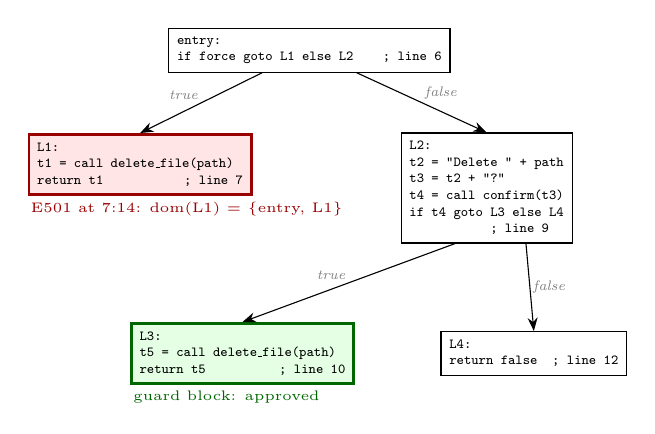
\begin{tikzpicture}[>=Stealth,
  blk/.style={draw, align=left, font=\ttfamily\tiny, inner sep=3pt, fill=white},
  bad/.style={blk, draw=red!60!black, fill=red!10, line width=0.9pt},
  guard/.style={blk, draw=green!40!black, fill=green!10, line width=0.9pt},
  lbl/.style={font=\tiny\itshape, text=gray, inner sep=1pt}]
\node[blk] (entry) at (0,0) {\textbf{entry:}\\if force goto L1 else L2 \ \ \ ; line 6};
\node[bad] (L1) at (-2.15,-1.45) {\textbf{L1:}\\t1 = call delete\_file(path)\\return t1 \ \ \ \ \ \ \ \ \ \ ; line 7};
\node[blk] (L2) at (2.25,-1.75) {\textbf{L2:}\\t2 = "Delete " + path\\t3 = t2 + "?"\\t4 = call confirm(t3)\\if t4 goto L3 else L4\\\hspace*{5.5em}; line 9};
\node[guard] (L3) at (-0.85,-3.85) {\textbf{L3:}\\t5 = call delete\_file(path)\\return t5 \ \ \ \ \ \ \ \ \ ; line 10};
\node[blk] (L4) at (2.85,-3.85) {\textbf{L4:}\\return false \ ; line 12};
\draw[->] ([xshift=-6mm]entry.south) -- node[lbl, above left] {true} (L1.north);
\draw[->] ([xshift=6mm]entry.south) -- node[lbl, above right] {false} (L2.north);
\draw[->] ([xshift=-4mm]L2.south) -- node[lbl, above left] {true} (L3.north);
\draw[->] ([xshift=5mm]L2.south) -- node[lbl, right] {false} (L4.north);
\node[anchor=north west, font=\tiny, text=red!60!black, inner sep=1pt] at ([yshift=-1pt]L1.south west) {E501 at 7:14: dom(L1) = \{entry, L1\}};
\node[anchor=north west, font=\tiny, text=green!40!black, inner sep=1pt] at ([yshift=-1pt]L3.south west) {guard block: approved};
\end{tikzpicture}
\caption{CFG of approval\_missing.as, drawn from compile -{}-phase cfg (one line note per block). L3 is the guard block; the call in L1 is not dominated by it.}
\label{fig:cfg}
\end{figure}

In \texttt{approval\_missing.as} (Fig.~\ref{fig:cfg}) the program deletes immediately when the parameter \texttt{force} is true and asks only on the other branch. The guard block is L3, which dominates the line 10 call; the line 7 call in L1 has dominators \{entry, L1\}, and no block with a \texttt{confirm} can reach it, so it is E501 (Fig.~\ref{fig:approval}). In \texttt{approval\_one\_branch.as} the confirmation is asked only when \texttt{careful} is true and its result is never branched on; the block of the confirm reaches the call after the \texttt{if}, so the code is E502 (Fig.~\ref{fig:e502}). In \texttt{valid\_cleanup.as}, which branches on \texttt{let ok = confirm(...)}, the report reads \texttt{delete\_file line 8 in L1: guarded by L1 -{}\textgreater{} approved}.

\begin{figure}[!htb]
\begin{lstlisting}
task purge
  dominators:
    entry  dom = {entry}  idom = -
    L1     dom = {entry, L1}  idom = entry
    L2     dom = {entry, L2}  idom = entry
    L3     dom = {entry, L2, L3}  idom = L2
    L4     dom = {entry, L2, L4}  idom = L2
  guard blocks:
    L3  (if confirm(...) on line 9; confirm on line 9)
  irreversible calls:
    delete_file line 7 in L1: guarded by - -> E501
    delete_file line 10 in L3: guarded by L3 -> approved

E501 [approval] 7:14: irreversible call to 'delete_file' (line 7) is reachable without confirm
    6:5  task purge starts (entry)
    6:5  line 6: if force -> true (L1)
    7:14  delete_file(...) is irreversible and not guarded by confirm
\end{lstlisting}
\caption{Approval report and E501 for approval\_missing.as (compile -{}-phase approval).}
\label{fig:approval}
\end{figure}

\begin{figure}[!htb]
\begin{lstlisting}
E502 [approval] 9:12: irreversible call to 'delete_file' (line 9) is not guarded by confirm on every path; the confirm on line 7 does not guard it
    6:5  task cleanup starts (entry)
    6:5  line 6: if careful -> false (L2)
    9:12  delete_file(...) is irreversible and not guarded by confirm
\end{lstlisting}
\caption{E502 for approval\_one\_branch.as (diagnostics section).}
\label{fig:e502}
\end{figure}

\section{Optimization and Code Generation}
\subsection{Optimizer}
The optimizer works on a deep copy of each CFG and runs four passes in a loop until a round changes nothing: (1) constant folding with block-local constant and copy propagation, turning a branch on a constant into a jump; (2) unreachable-block elimination; (3) dead-assignment elimination, which never removes a \texttt{Call} (a side effect and a budget unit) or an \texttt{Index} (it may raise E603); and (4) duplicate tool-call elimination. The last pass replaces a call to a \texttt{mergeable} tool by a copy of an earlier result only within one basic block, with identical operands, no other call in between and no redefinition of the arguments; it never applies to \texttt{send\_email}, \texttt{delete\_file} or \texttt{confirm}, since merging a side effect or a human approval would change what the agent does.

Fig.~\ref{fig:optsrc} shows the task of \texttt{optimize\_demo.as} and Fig.~\ref{fig:opt} the real report: tool calls go from 4 to 2 and instructions from 14 to 10. One \texttt{web\_search} is merged (\texttt{again = first} is kept because \texttt{again[2]} still reads it) and the debug \texttt{llm} disappears with its unreachable block. The checks are not re-run, yet they still hold: calls are only removed or merged, so the budget bound remains valid; no new data flow is created; and no call moves between blocks while only unreachable blocks are deleted, which can only strengthen dominance.

\begin{figure}[!htb]
\begin{lstlisting}
  task research(topic: string) -> string {
    let pages = 2 * 3;
    let first = web_search(topic);
    let again = web_search(topic);
    let debug = false;
    if (debug) {
      return llm("debug");
    }
    return llm("Compare: " + first[1] + " / " + again[2]);
  }
\end{lstlisting}
\caption{The task of examples/optimize\_demo.as.}
\label{fig:optsrc}
\end{figure}

\begin{figure}[!htb]
\begin{lstlisting}
instructions 14 -> 10, tool calls 4 -> 2
changes:
  line 6: folded pages = 2 * 3 -> 6
  line 10: replaced debug with false
  line 10: branch on false -> goto L2
  removed unreachable block L1 (line 11)
  line 6: removed dead assignment pages = 6
  line 9: removed dead assignment debug = false
  line 8: duplicate call web_search(topic) replaced by copy of first (line 7)
\end{lstlisting}
\caption{End of compile -{}-phase optimized\_ir for optimize\_demo.as.}
\label{fig:opt}
\end{figure}

\subsection{Bytecode and Virtual Machine}
Code generation lowers each three-address instruction to ``push the operands, operate, store'' for a stack machine with the opcodes \texttt{PUSH\_CONST}, \texttt{LOAD}, \texttt{STORE}, \texttt{ADD}, \texttt{SUB}, \texttt{MUL}, six comparisons, \texttt{INDEX}, \texttt{CALL tool argc}, \texttt{CALL\_PARALLEL}, \texttt{JUMP}, \texttt{JUMP\_IF\_FALSE} and \texttt{RETURN}. Blocks are laid out in CFG order, jumps to the next block are omitted and forward jumps are backpatched in a second pass. For \texttt{valid\_report.as} the result is 30 instructions without a single \texttt{JUMP} (Fig.~\ref{fig:bytecode}).

\begin{figure}[!htb]
\begin{lstlisting}
agent Assistant  permit [web_search, llm, sanitize, send_email, confirm]  budget 5
task report(topic: string) -> bool
    0  LOAD topic                     ; line 6
    1  CALL web_search 1              ; line 6
    2  STORE raw                      ; line 6
...
   17  PUSH_CONST "Send report?"      ; line 9
   18  CALL confirm 1                 ; line 9
   19  STORE t3                       ; line 9
   20  LOAD t3                        ; line 9
   21  JUMP_IF_FALSE 28               ; line 9
   22  PUSH_CONST "me@example.com"    ; line 10
   23  LOAD summary                   ; line 10
   24  CALL send_email 2              ; line 10
   25  STORE t4                       ; line 10
   26  LOAD t4                        ; line 10
   27  RETURN                         ; line 10
   28  PUSH_CONST false               ; line 12
   29  RETURN                         ; line 12
\end{lstlisting}
\caption{Bytecode of valid\_report.as (compile -{}-phase bytecode, cut).}
\label{fig:bytecode}
\end{figure}

The program carries its permits and budget, so the VM enforces them without trusting the compiler. Before every call it checks the budget (E601) and the permission list (E602); \texttt{INDEX} checks bounds (E603); arguments are validated against the task signature before the first instruction (E604); and a run stops after 1,000,000 executed instructions (E601), because the call budget does not bound call-free loops. Tools come from a deterministic mock registry by default, whose \texttt{web\_search} deliberately returns an injection string; an optional live mode uses real \texttt{llm} and \texttt{web\_search} services, while \texttt{send\_email} and \texttt{delete\_file} are always simulated. Table~\ref{tab:runlog} summarizes the real run of the example with \texttt{\{\textquotedbl{}topic\textquotedbl{}: \textquotedbl{}AI safety\textquotedbl{}\}}: 5 calls of the budget of 5, value \texttt{true}; call 2 shows \texttt{sanitize} replacing the injected instruction with ``[removed instruction]''. Fig.~\ref{fig:e601} shows the runtime guard on \texttt{runtime\_budget.as} with \texttt{times = 5}: the fourth call is never made.

\begin{table}[!htb]
\caption{Call Log of the Mock Run of valid\_report.as}
\label{tab:runlog}
\centering
\footnotesize
\setlength{\tabcolsep}{3pt}
\renewcommand{\arraystretch}{1.1}
\begin{tabular}{P{0.165in}P{0.365in}P{0.265in}P{0.765in}P{1.515in}}
\hline
\textbf{\#} & \textbf{Round} & \textbf{Line} & \textbf{Tool} & \textbf{Result (cut)} \\
\hline
1 & 1 & 6 & \texttt{web\_search} & list of 3 strings \\
2 & 2 & 7 & \texttt{sanitize} & \texttt{\textquotedbl{}AI safety: [removed instruction] ...} \\
3 & 3 & 8 & \texttt{llm} & \texttt{\textquotedbl{}[llm] Summarize: AI safety: ...} \\
4 & 4 & 9 & \texttt{confirm} & \texttt{true} \\
5 & 5 & 10 & \texttt{send\_email} & \texttt{true} \\
\hline
\end{tabular}
\end{table}
\begin{figure}[!htb]
\begin{lstlisting}
W306 [semantic] 6:12: repeat count 'times' is not a literal; the budget for this loop is enforced at runtime
calls: 3 of budget 3
...
E601 [runtime] 7:15: budget exceeded: call 4 would exceed the budget of 3 calls
\end{lstlisting}
\caption{Run of runtime\_budget.as with times = 5 (call log cut).}
\label{fig:e601}
\end{figure}

\subsection{Parallel Scheduling}
The optional scheduler builds a dependency graph per basic block of the optimized IR. Data edges join instructions that read or write the same variable; \emph{barrier} edges keep every call to a \texttt{privileged}, \texttt{irreversible} or \texttt{approval} tool in order relative to every other call; and an \texttt{Index} is ordered against every call because it may fail. List scheduling then emits all ready non-call instructions, followed by all ready calls as one round. A round of two or more calls becomes one \texttt{CALL\_PARALLEL}, which the VM runs on a thread pool and logs in program order. The guards are checked per call in program order, so a run that fails inside a round makes exactly the calls that the sequential program would. In \texttt{parallel\_demo.as} the three independent searches share round 1 and the rounds drop from 4 to 2 (Fig.~\ref{fig:sched}); in \texttt{valid\_report.as} every call depends on the previous one and the rounds stay at 5.

\begin{figure}[!htb]
\begin{lstlisting}
task scout: rounds 4 -> 2
  entry:
    round 1: ra = call web_search(a) | rb = call web_search(b) | rc = call web_search(c)
    round 2: t8 = call llm(t7)
total: rounds 4 -> 2

    0  LOAD a                         ; line 6
    1  LOAD b                         ; line 7
    2  LOAD c                         ; line 8
    3  CALL_PARALLEL web_search/1, web_search/1, web_search/1 ; line 6
    4  STORE rc                       ; line 8
    5  STORE rb                       ; line 7
    6  STORE ra                       ; line 6
...
\end{lstlisting}
\caption{Schedule of parallel\_demo.as (compile -{}-phase schedule) and the start of its bytecode.}
\label{fig:sched}
\end{figure}

\section{Implementation and Editor}
The compiler and VM are written in Python 3.12 with only the standard library; the server uses FastAPI~\cite{fastapi} with uvicorn, and the tests use pytest and httpx. The package \texttt{agentscript/\allowbreak{}} has 22 Python files with 5008 lines (Table~\ref{tab:modules}). \texttt{pipeline.py} runs the stages in order and never raises: a phase error becomes a diagnostic and later artifacts stay \texttt{null}. Because the phases recurse over the AST, compilation runs in a worker thread with a large stack and a raised recursion limit. The command line offers \texttt{compile} (with \texttt{-{}-{}phase} for one artifact and \texttt{-{}-{}json} for the full response), \texttt{run} (with \texttt{-{}-{}deny-{}confirm} and \texttt{-{}-{}live}) and \texttt{serve}.

\begin{table}[!htb]
\caption{Pipeline Stages, Modules and Artifact Keys}
\label{tab:modules}
\centering
\footnotesize
\setlength{\tabcolsep}{3pt}
\renewcommand{\arraystretch}{1.1}
\begin{tabular}{P{0.165in}P{0.965in}P{1.165in}P{0.865in}}
\hline
\textbf{\#} & \textbf{Stage} & \textbf{Module(s)} & \textbf{Artifact} \\
\hline
1 & Lexer & \texttt{lexer.py} & \texttt{tokens} \\
2 & Parser & \texttt{parser.py}, \texttt{ast\_nodes.py} & \texttt{ast} \\
3 & Semantic & \texttt{semantic.py}, \texttt{typesys.py}, \texttt{tools.py} & \texttt{symbols} \\
4 & IR + CFG & \texttt{irgen.py}, \texttt{ir.py}, \texttt{cfg.py} & \texttt{ir}, \texttt{cfg} \\
5 & Taint & \texttt{taint.py} & \texttt{taint} \\
6 & Approval & \texttt{approval.py} & \texttt{approval} \\
7 & Optimizer & \texttt{optimizer.py} & \texttt{optimized\_ir} \\
8 & Scheduler & \texttt{scheduler.py} & \texttt{schedule} \\
9 & Codegen & \texttt{codegen.py}, \texttt{bytecode.py} & \texttt{bytecode} \\
10 & VM & \texttt{vm.py}, \texttt{registry.py} & run result \\
\hline
\end{tabular}
\end{table}
The API exposes \texttt{GET /\allowbreak{}} (the editor), \texttt{GET /\allowbreak{}examples} (the 18 manifest entries with their sources), \texttt{POST /\allowbreak{}compile} (every artifact, the diagnostics, before/after counts and task signatures) and \texttt{POST /\allowbreak{}run} (value, call log, calls used and budget). The editor is one static page in vanilla JavaScript with CodeMirror 5 and Mermaid from a CDN and no build tooling (\texttt{web/\allowbreak{}}: 3328 lines). A pipeline strip shows one status chip per stage; tabs show Tokens, AST, Symbols, Errors, IR, CFG (drawn with Mermaid), Taint, Approval, Optimized IR, Rounds, Bytecode and Output. Diagnostics become squiggles and gutter markers, tainted lines are tinted, path steps are clickable, and a run panel offers a task picker, JSON arguments, an Approve/Deny switch for \texttt{confirm} and a live-tools toggle.

\section{Evaluation}
\subsection{Test Suite}
The command \texttt{.venv/\allowbreak{}bin/\allowbreak{}pytest -{}q} ends with \texttt{941 passed,\allowbreak{} 11 skipped in 9.48s}. Pytest collects 952 tests in 16 files (Table~\ref{tab:tests}); the 11 skips are parametrized cases that do not apply (9 manifest examples that fail before the approval stage, and 2 lexical-error examples that the lexer tests cover). Besides unit tests per phase, golden tests compare every phase text and the diagnostics of each of the 18 examples with \texttt{tests/\allowbreak{}golden/\allowbreak{}\textless{}example\textgreater{}.json}, which is stable because the mock tools are deterministic; negative tests check the code, line and column of every failing example against \texttt{examples/\allowbreak{}manifest.json}; and end-to-end, CLI and API tests exercise the whole pipeline.

\begin{table}[!htb]
\caption{Collected Tests per File (952 in Total)}
\label{tab:tests}
\centering
\footnotesize
\setlength{\tabcolsep}{3pt}
\renewcommand{\arraystretch}{1.1}
\begin{tabular}{P{1.265in}P{0.315in}P{1.265in}P{0.315in}}
\hline
\textbf{File} & \textbf{Tests} & \textbf{File} & \textbf{Tests} \\
\hline
\texttt{test\_lexer.py} & 74 & \texttt{test\_optimizer.py} & 61 \\
\texttt{test\_parser.py} & 107 & \texttt{test\_scheduler.py} & 41 \\
\texttt{test\_semantic.py} & 105 & \texttt{test\_codegen.py} & 55 \\
\texttt{test\_irgen.py} & 48 & \texttt{test\_vm.py} & 97 \\
\texttt{test\_cfg.py} & 43 & \texttt{test\_registry.py} & 26 \\
\texttt{test\_taint.py} & 43 & \texttt{test\_pipeline.py} & 105 \\
\texttt{test\_approval.py} & 44 & \texttt{test\_cli.py} & 27 \\
\texttt{test\_golden.py} & 37 & \texttt{test\_api.py} & 39 \\
\hline
\end{tabular}
\end{table}
\subsection{Error Taxonomy}
Each phase owns a class of errors and each class has a failing demo program, so an evaluator can watch every phase catch its own mistakes. Table~\ref{tab:errors} lists the codes. Running \texttt{compile} on each example reproduces the code and location recorded in the manifest; the runtime codes are reproduced by \texttt{run} with the manifest's arguments. E602 cannot be reached by compiled programs, because E305 rejects them first, so it is tested with hand-made bytecode; E604 concerns the run request, not the source, and is reported at 0:0.

\begin{table}[!htb]
\caption{Error Taxonomy (Locations from examples/manifest.json)}
\label{tab:errors}
\centering
\footnotesize
\setlength{\tabcolsep}{3pt}
\renewcommand{\arraystretch}{1.1}
\begin{tabular}{P{0.365in}P{0.565in}P{1.715in}P{0.515in}}
\hline
\textbf{Code} & \textbf{Phase} & \textbf{Demo program} & \textbf{Line:col} \\
\hline
E101 & lexer & \texttt{lex\_unterminated.as} & 6:13 \\
E102 & lexer & \texttt{lex\_illegal\_char.as} & 6:15 \\
E201 & parser & \texttt{syntax\_missing\_semicolon.as} & 6:30 \\
E301 & semantic & \texttt{sem\_undeclared.as} & 6:12 \\
E302 & semantic & \texttt{sem\_duplicate.as} & 7:9 \\
E303 & semantic & \texttt{sem\_type\_mismatch.as} & 6:23 \\
E304 & semantic & \texttt{sem\_missing\_return.as} & 9:3 \\
E305 & semantic & \texttt{sem\_not\_permitted.as} & 6:16 \\
E306 & semantic & \texttt{sem\_budget.as} & 9:12 \\
W306 & semantic & \texttt{runtime\_budget.as} & 6:12 \\
E401 & taint & \texttt{taint\_injection.as} & 9:14 \\
E501 & approval & \texttt{approval\_missing.as} & 7:14 \\
E502 & approval & \texttt{approval\_one\_branch.as} & 9:12 \\
E601 & runtime & \texttt{runtime\_budget.as} (run) & 7:15 \\
E602 & runtime & unit test (hand-made bytecode) & -- \\
E603 & runtime & \texttt{runtime\_index.as} (run) & 7:19 \\
E604 & runtime & VM and API tests & 0:0 \\
\hline
\end{tabular}
\end{table}
\subsection{Success Metrics}
Table~\ref{tab:metrics} compares the targets of the specification with the measured results; every target is met, including the stretch goal of parallel rounds.

\begin{table}[!htb]
\caption{Success Metrics: Target and Measured Result}
\label{tab:metrics}
\centering
\footnotesize
\setlength{\tabcolsep}{3pt}
\renewcommand{\arraystretch}{1.1}
\begin{tabular}{P{1.065in}P{1.015in}P{1.165in}}
\hline
\textbf{Metric} & \textbf{Target} & \textbf{Result} \\
\hline
Classic phases visible in the editor & 6 of 6; a tab per stage & 6 of 6; all 10 stages have a tab \\
Error types, each with a failing program & at least 8 & 14 codes with demos, plus W306; E602, E604 by tests \\
Injection example & rejected at compile time & E401 at 9:14 \\
Unapproved irreversible call & rejected at compile time & E501 at 7:14, E502 at 9:12 \\
Optimizer demo & duplicate call removed & calls 4 $\rightarrow$ 2, instructions 14 $\rightarrow$ 10 \\
Parallel rounds (stretch) & 3 calls in 1 round & rounds 4 $\rightarrow$ 2 \\
\hline
\end{tabular}
\end{table}
\section{Limitations and Future Work}
The analyses are conservative and their assumptions are stated openly. Taint tracks explicit flows only: \texttt{if (raw[0] == \textquotedbl{}yes\textquotedbl{}) \{ send\_email(to,\allowbreak{} \textquotedbl{}it said yes\textquotedbl{}); \}} leaks one bit through the branch decision. A list has one label, task parameters are trusted, and \texttt{sanitize} is trusted by definition, so the compiler proves that sanitizing happens, not that the sanitizer is perfect. The analysis follows data, not model behaviour: \texttt{llm} of trusted text is assumed trusted, and \texttt{llm} can never clear taint. The static budget ignores early returns and takes the larger branch, so a program that could never exceed its budget may be rejected. Approval needs a single dominating guard: two confirmations on two branches before a join are rejected with E502, \texttt{confirm(...) == true} is not accepted, and one confirmation before a \texttt{repeat} approves every iteration. Only the first error is reported, propagation is block-local, only adjacent duplicate calls are merged, mergeable tools are assumed deterministic within a run, and there is no bytecode verifier.

Natural extensions are implicit-flow tracking with a program-counter label~\cite{denning}, \cite{sabelfeld}, a richer label lattice per source, global duplicate-call elimination based on available expressions~\cite{aho}, faster dominator algorithms~\cite{lt}, \cite{cooper} for larger programs, parser error recovery, and reviewed user-declared tools. Task-to-task calls would require interprocedural versions of both analyses.

\section{Conclusion}
AgentScript shows that textbook compiler techniques catch real agent-safety bugs before any tool fires: a forward data-flow analysis rejects the prompt-injection flow of \texttt{taint\_injection.as} (E401 at 9:14), and dominators over guard blocks reject unapproved deletions (E501 at 7:14, E502 at 9:12). Running every safety analysis on the unoptimized program keeps the guarantees independent of the optimizer, which still removes half of the tool calls of its demo program, and the runtime guards of the VM cover what static analysis cannot know. The whole pipeline, from tokens to the call log, is visible in a web editor and covered by 941 passing tests.

\begin{thebibliography}{00}
\bibitem{greshake} K. Greshake, S. Abdelnabi, S. Mishra, C. Endres, T. Holz, and M. Fritz, ``Not what you've signed up for: Compromising real-world LLM-integrated applications with indirect prompt injection,'' in \emph{Proc. 16th ACM Workshop Artif. Intell. Secur. (AISec)}, 2023, pp. 79--90.
\bibitem{owasp} OWASP Foundation, ``OWASP Top 10 for large language model applications,'' 2023. [Online]. Available: \url{https://owasp.org/www-project-top-10-for-large-language-model-applications/}
\bibitem{aho} A. V. Aho, M. S. Lam, R. Sethi, and J. D. Ullman, \emph{Compilers: Principles, Techniques, and Tools}, 2nd ed. Boston, MA, USA: Addison-Wesley, 2006.
\bibitem{dspy} O. Khattab \emph{et al.}, ``DSPy: Compiling declarative language model calls into self-improving pipelines,'' in \emph{Proc. Int. Conf. Learn. Represent. (ICLR)}, 2024.
\bibitem{lmql} L. Beurer-Kellner, M. Fischer, and M. Vechev, ``Prompting is programming: A query language for large language models,'' \emph{Proc. ACM Program. Lang.}, vol. 7, no. PLDI, 2023, Art. no. 186.
\bibitem{guidance} Guidance contributors, ``Guidance: A guidance language for controlling large language models,'' GitHub repository. [Online]. Available: \url{https://github.com/guidance-ai/guidance}
\bibitem{baml} Boundary, ``BAML: A domain-specific language for structured LLM functions,'' GitHub repository. [Online]. Available: \url{https://github.com/BoundaryML/baml}
\bibitem{camel} E. Debenedetti \emph{et al.}, ``Defeating prompt injections by design,'' 2025, \emph{arXiv:2503.18813}.
\bibitem{denning} D. E. Denning, ``A lattice model of secure information flow,'' \emph{Commun. ACM}, vol. 19, no. 5, pp. 236--243, May 1976.
\bibitem{sabelfeld} A. Sabelfeld and A. C. Myers, ``Language-based information-flow security,'' \emph{IEEE J. Sel. Areas Commun.}, vol. 21, no. 1, pp. 5--19, Jan. 2003.
\bibitem{jflow} A. C. Myers, ``JFlow: Practical mostly-static information flow control,'' in \emph{Proc. 26th ACM SIGPLAN-SIGACT Symp. Princ. Program. Lang. (POPL)}, 1999, pp. 228--241.
\bibitem{livshits} V. B. Livshits and M. S. Lam, ``Finding security vulnerabilities in Java applications with static analysis,'' in \emph{Proc. 14th USENIX Secur. Symp.}, 2005, pp. 271--286.
\bibitem{allen} F. E. Allen, ``Control flow analysis,'' \emph{ACM SIGPLAN Notices}, vol. 5, no. 7, pp. 1--19, Jul. 1970.
\bibitem{kildall} G. A. Kildall, ``A unified approach to global program optimization,'' in \emph{Proc. 1st ACM SIGACT-SIGPLAN Symp. Princ. Program. Lang. (POPL)}, 1973, pp. 194--206.
\bibitem{lt} T. Lengauer and R. E. Tarjan, ``A fast algorithm for finding dominators in a flowgraph,'' \emph{ACM Trans. Program. Lang. Syst.}, vol. 1, no. 1, pp. 121--141, Jul. 1979.
\bibitem{cooper} K. D. Cooper, T. J. Harvey, and K. Kennedy, ``A simple, fast dominance algorithm,'' Dept. Comput. Sci., Rice Univ., Houston, TX, USA, Tech. Rep., 2001.
\bibitem{dennis} J. B. Dennis and E. C. Van Horn, ``Programming semantics for multiprogrammed computations,'' \emph{Commun. ACM}, vol. 9, no. 3, pp. 143--155, Mar. 1966.
\bibitem{miller} M. S. Miller, ``Robust composition: Towards a unified approach to access control and concurrency control,'' Ph.D. dissertation, Johns Hopkins Univ., Baltimore, MD, USA, 2006.
\bibitem{lucassen} J. M. Lucassen and D. K. Gifford, ``Polymorphic effect systems,'' in \emph{Proc. 15th ACM SIGPLAN-SIGACT Symp. Princ. Program. Lang. (POPL)}, 1988, pp. 47--57.
\bibitem{fastapi} S. Ram\'{\i}rez, ``FastAPI,'' [Online]. Available: \url{https://fastapi.tiangolo.com}
\end{thebibliography}

\end{document}
